\documentclass{beamer}


\usepackage[utf8]{inputenc}

\usepackage{pgffor}
\usepackage{graphicx}
\usepackage{caption}
\usepackage{eso-pic}
\usepackage{datetime}
\usepackage{hyperref}
\usepackage{datetime}
\usepackage{colortbl}
\usepackage{minted}
\usepackage{ulem}
% \usepackage[table]{xcolor}% http://ctan.org/pkg/xcolor


% \usepackage{movie15}
\usetheme{metropolis}

\newdate{date}{26}{12}{2021}


% \author{\textbf{}
\institute{Inria Rennes}
\date{\displaydate{date}}
\date{2022-11-21}
\title[Bonnes pratique logicielles, test unitaires etc.]{Bonnes pratique logicielles, test unitaires etc.}

% \AtBeginSection[]
% {
%     \begin{frame}
%         \frametitle{Summary}
%         \tableofcontents[currentsection]
%     \end{frame}
% }
 
\begin{document}
\setbeamertemplate{footline}[frame number]
\frame{\titlepage}


% automatic table of content at every section
% \begin{frame}
%     \tableofcontents[pausesections]
% \end{frame}

\section{Constat sur les codes en recherche}
\begin{frame}
    \frametitle{Constat sur les codes en recherche}
    On n'écrit pas de code pour des clients, on écrit du code pour des reviewers (pas la même notion de durée).\\
    \begin{itemize}
        \item on part d'une idée pré-éxistante
        \item on code
        \item on modifie l'idée de départ
        \item on modifie le code
        \item on répete
        \item on publie
        \item (on oublie)
    \end{itemize}
\end{frame}


% \section{Conséquence de la méthodologie}
\begin{frame}
    \frametitle{Conséquence de la méthodologie}
    Pas de mises à jour $\implies $un bug a tendance à rester.\\

    De nouveaux bugs peuvent aussi apparaitre, ex:% au fur et à mesure des mises à jour des machines, il est difficile de savoir si un outil va fonctionner correctement.

    % Ex:
    \begin{itemize}
        \item python 3.10 n'autorise plus l'affichage de grand nombre
        \item le passage de PHP 7.3 à 7.4 introduit un nouveau mot-clef et n'installe plus PEAR par défaut
    \end{itemize}
\end{frame}

\section{Architecture logicielle}
\begin{frame}
    \frametitle{Architecture logicielle}

    La plus facile à mettre en oeuvre sur les langage orienté objet est la l'architecture ``orientée objets''.\\

    Un des principe clef en est l'\textbf{encapsulation}.\\

    Chaque composant n'expose que le minimum nécessaire.\\

    Pensez à bien nommer vos composants!



\end{frame}

\begin{frame}
    \frametitle{Architecture logicielle}

    Ne pas faire:\\
    \inputminted{cpp}{../code/cpp/Parent.cpp}

\end{frame}

\begin{frame}
    \frametitle{Architecture logicielle}

    Ne pas faire:\\
    \inputminted{cpp}{../code/cpp/Enfant.cpp}

\end{frame}

\begin{frame}
    \frametitle{Architecture logicielle}

    Faire:\\
    \inputminted{cpp}{../code/cpp/Parent_ok.cpp}

\end{frame}

\begin{frame}
    \frametitle{Architecture logicielle}

    Faire:\\
    \inputminted{cpp}{../code/cpp/Enfant_ok.cpp}

\end{frame}

\section{Utilisation des langages}
\begin{frame}
    \frametitle{Un peu de python}
    \inputminted{python}{../code/python/intro/intro.py}
    Seems OK, but:
    \begin{itemize}
        \item no type annotation
        \item no error handling
        \item no documentation
    \end{itemize}
    % \end{columns}
\end{frame}

\begin{frame}
    \frametitle{Un peu de python}
    \inputminted{python}{../code/python/intro/intro_annotated.py}
    Seems OK, but:
    \begin{itemize}
        \item \sout{type annotation}
        \item no error handling
        \item no documentation
    \end{itemize}
\end{frame}

\begin{frame}
    \frametitle{Un peu de python}
    \inputminted{python}{../code/python/intro/intro_annotated_error.py}
    Seems OK, but:
    \begin{itemize}
        \item \sout{type annotation}
        \item \sout{no error handling}
        \item no documentation
    \end{itemize}
\end{frame}

\begin{frame}
    \frametitle{Un peu de python}
    \inputminted{python}{../code/python/intro/intro_annotated_error_doc.py}
    Perfection !
\end{frame}

\section{Des ribambelles de tests}




\begin{frame}
    \frametitle{Pourquoi tester ? Ça se voit que ça marche}
    \inputminted{python}{../code/python/intro/tuple_assign.py}
\end{frame}


\begin{frame}
    \frametitle{Pourquoi tester ? Ça se voit que ça marche}
    \inputminted{python}{../code/python/intro/__main__.py}
\end{frame}

\begin{frame}
    \frametitle{Pourquoi tester ? Ça se voit que ça marche}
    $tuple\_integer\ before += : (0,)$\\
    'tuple' object does not support item assignment\\
    $tuple\_integer\ after += : (0,)$\\

    $tuple\_list\ before += : ([],)$\\
    'tuple' object does not support item assignment\\
    $tuple\_list\ after += : (['truc'],)$
\end{frame}

\begin{frame}
    \frametitle{Pourquoi tester ? Ça se voit que ça marche}
    \inputminted{python}{../code/python/intro/def_arg_0.py}
\end{frame}

\begin{frame}
    \frametitle{Pourquoi tester ? Ça se voit que ça marche}
    \inputminted{python}{../code/python/intro/def_arg_1.py}
\end{frame}

\begin{frame}
    \frametitle{Pourquoi tester ? Ça se voit que ça marche}
    \inputminted{python}{../code/python/intro/def_arg_2.py}
    \begin{columns}
        \column{0.5\textwidth}
        \column{0.5\textwidth}
        \begin{figure}
            
\includegraphics[width=5cm]{img/horror.jpg}
        \end{figure}
    \end{columns}
\end{frame}


\begin{frame}
    \frametitle{OK, OK... Comment je vérifie mon programme ?}
    Par des tests !

    \begin{itemize}
        \item tests unitaires
        \item tests d'intégration
        \item tests de validation
    \end{itemize}
\end{frame}


\begin{frame}
    \frametitle{Tests unitaires}
    Le but est de vérifier le comportement de chaque unité de code, indépendamment des autres unités.\\
    Il existe généralement des solutions pour chaque langage.\\
\end{frame}

\begin{frame}
    \frametitle{Tests unitaires}
    L'utilisation de bout de code "inutiles" (les mocks) est possible pour isoler les unités à tester.
    \begin{figure}
        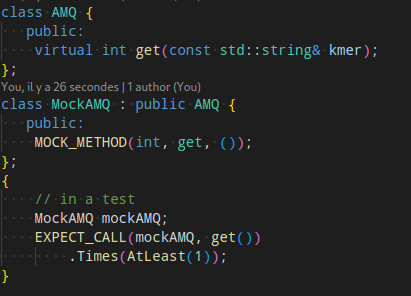
\includegraphics[width=8cm]{img/mock.png}
    \end{figure}
\end{frame}

\begin{frame}
    \frametitle{Tests unitaires (C++)}
    \begin{figure}
        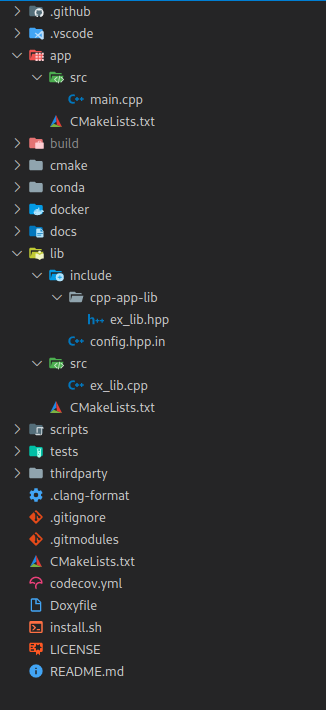
\includegraphics[width=5cm]{img/arbre.png}
    \end{figure}
\end{frame}

\begin{frame}
    \frametitle{Tests d'intégration}
    Le but est de vérifier le comportement du programme total, en utilisant un maximum d'unités.\\
    Cela permet de detecter des erreurs de communication entre les unités ou de détecter des API cassées.\\
\end{frame}


\begin{frame}
    \frametitle{Tests d'intégration}
    \begin{figure}
        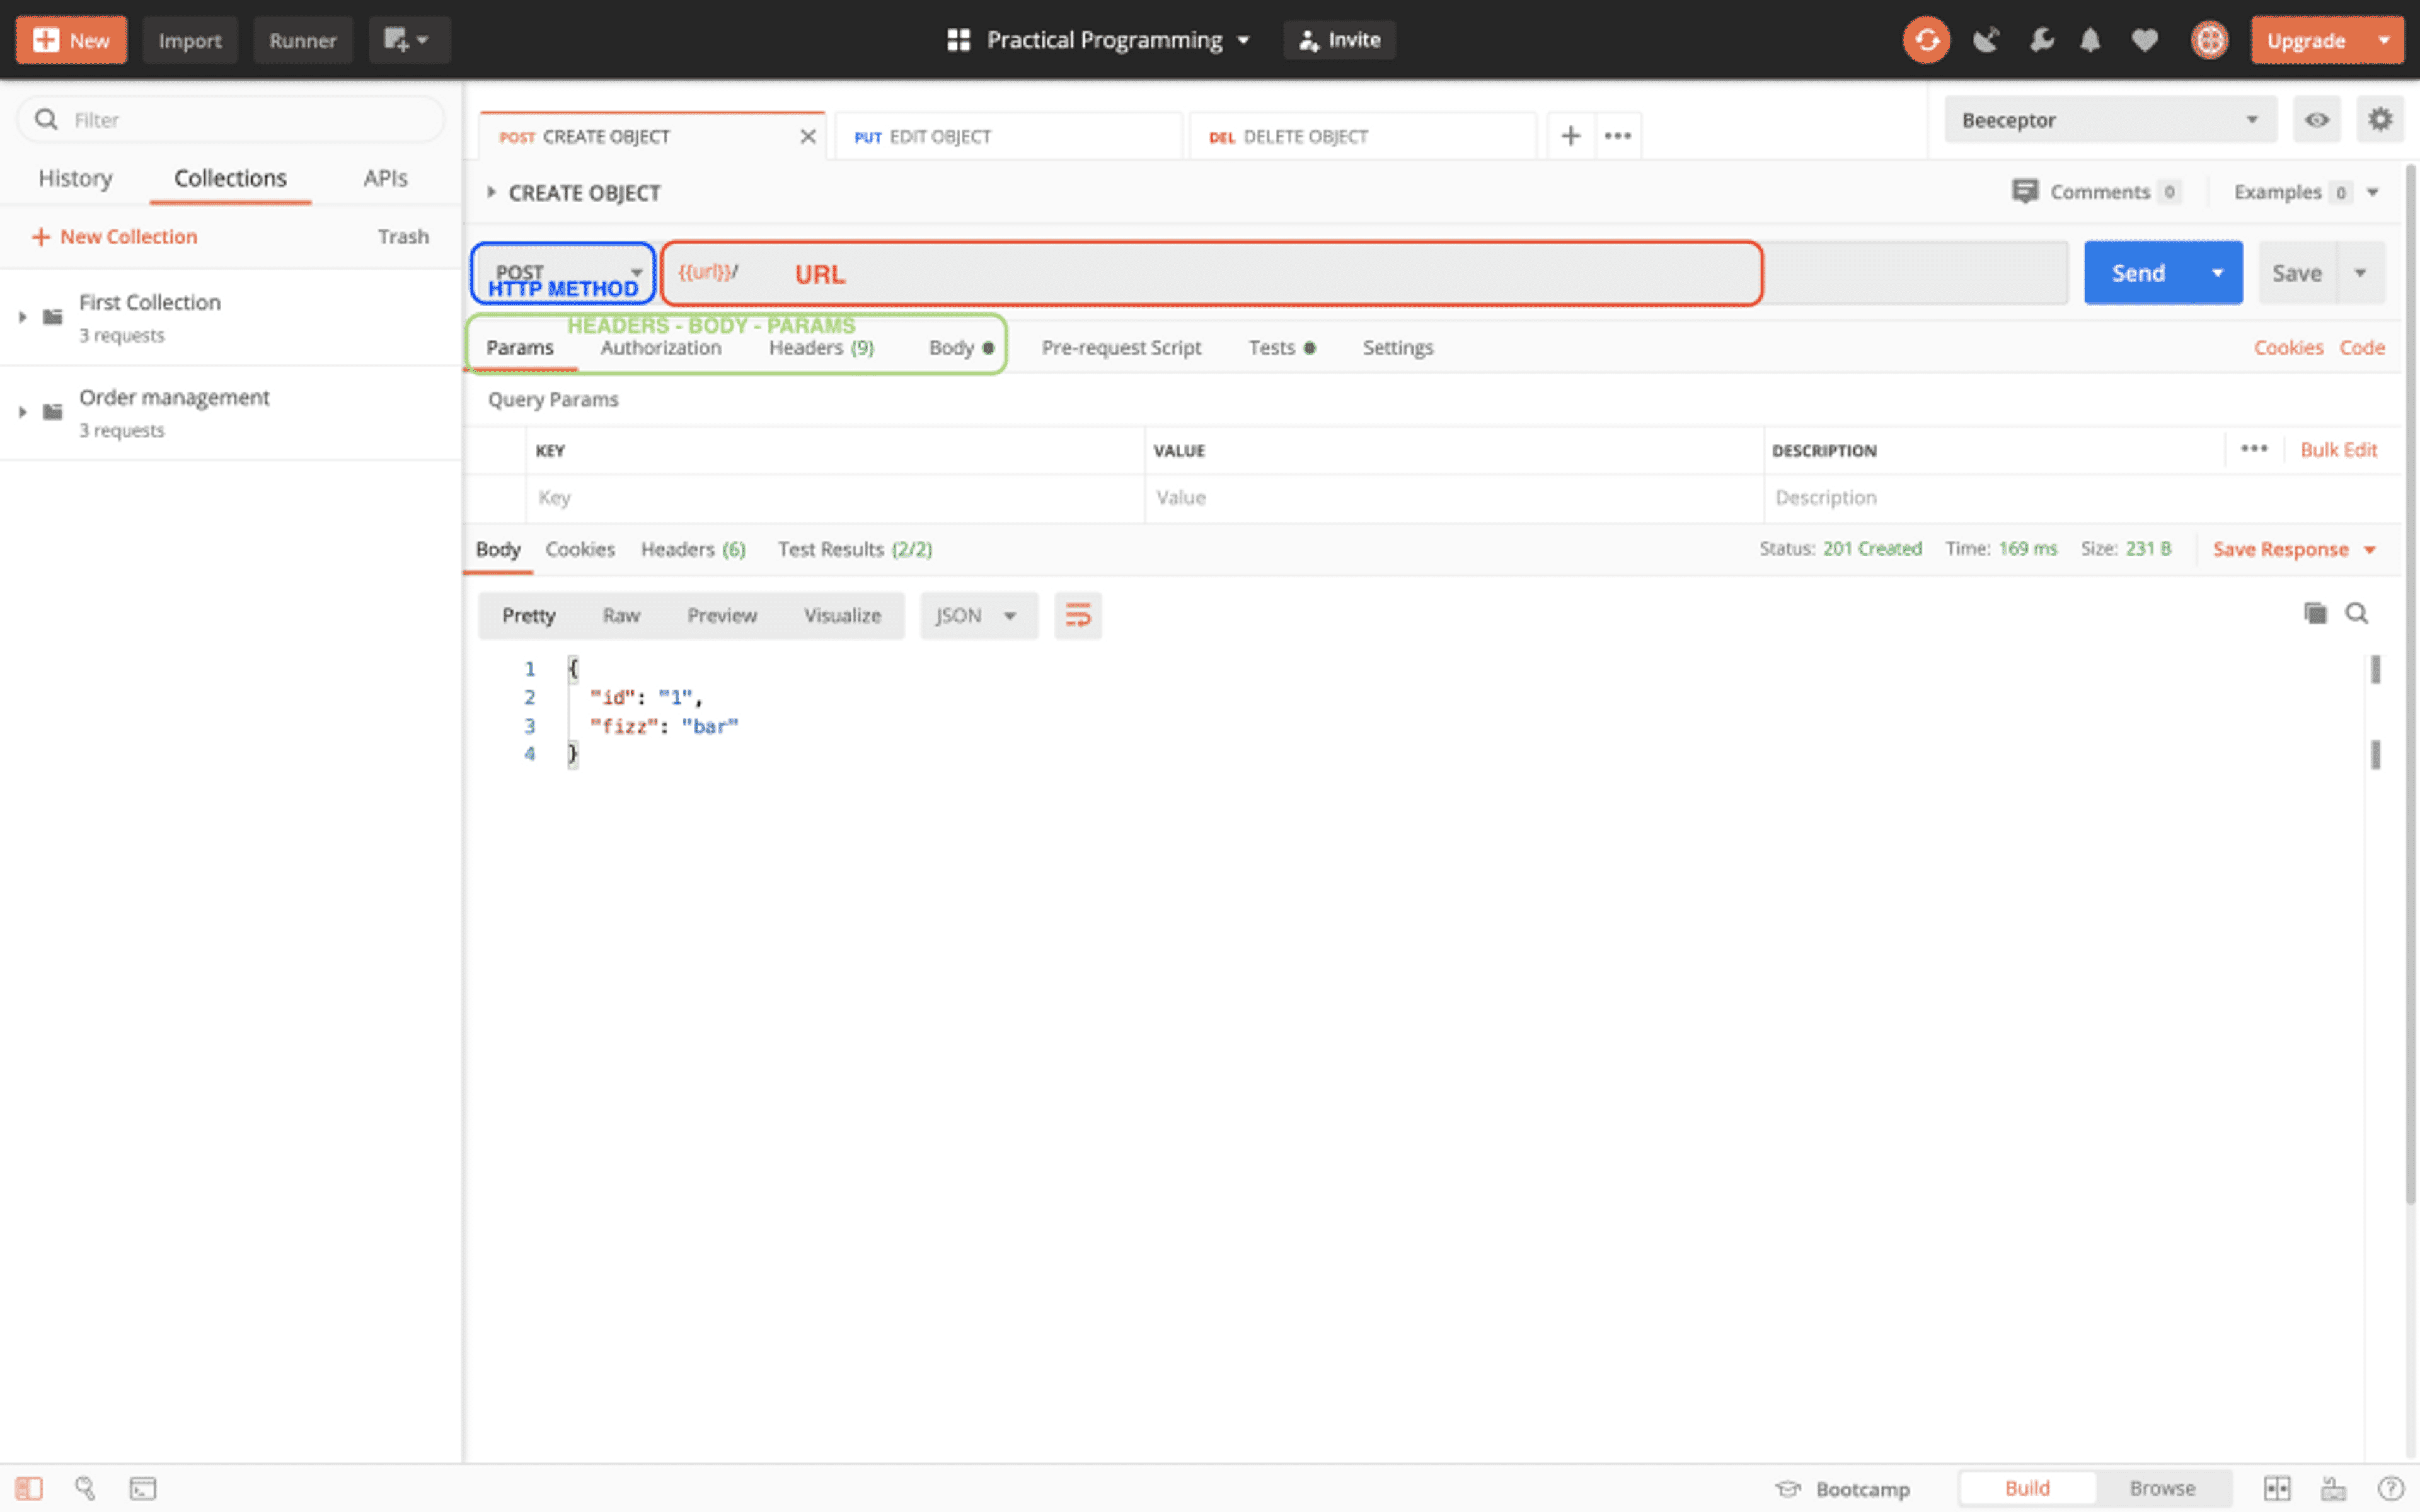
\includegraphics[width=11cm]{img/postman.png}
    \end{figure}
\end{frame}

\begin{frame}
    \frametitle{Tests de validation}
    \begin{itemize}
        \item scénarios d'utilisation concrète
        \item simule ce qu'un reviewer ferait pour rapidemment voir que ``ça marche''
    \end{itemize}
    C'est aussi à cette étape que sont réalisés les tests de performance par exemple.
\end{frame}

\begin{frame}
    \frametitle{Quelques petites remarques:}
    Tester est chronophage (en particulier, l'utilisation de mock).\\
    Préférer tester les plus petites unités d'abord, puis remonter l'arbre de dépendance.\\
    $\implies$ fusion des tests unitaires et d'intégration.
\end{frame}

\begin{frame}
    \frametitle{Quelques petites remarques:}
    \begin{figure}
        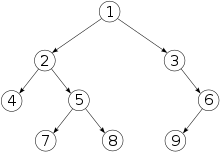
\includegraphics[width=8cm]{img/arbre_dep.png}
        \caption{proposition d'ordre: {4, 7, 8, 9}, puis {2, 5, 6}, puis 3 puis 1}
    \end{figure}
\end{frame}

\begin{frame}
    \frametitle{Les chaines CICD}
    Outil permettant:
    \begin{itemize}
        \item de compiler le code à chaque mises à jour
        \item d'exécuter les tests
        \item de mettre à disposition des rapports
    \end{itemize}
\end{frame}

\end{document}